\chapter{Modelagem Híbrida}\label{Desenvolvimento} 

Afim de se cumprir com o objetivo principal de desenvolver e validar uma metodologia de modelagem híbrida baseada em Processamento de Linguagem Natural (PLN) que combine análise de sentimentos, modelagem de tópicos e técnicas de clusterização para análise de publicações e comentários de redes sociais, este projeto aplciado em dados do Instagram inicia-se com um pipeline de Extração, Transformação e Carga (ETL) automatizado, que utiliza a API da Apify para coletar dados de perfis, postagens e reels de governadores. Na fase de transformação, os dados brutos são enriquecidos com métricas de engajamento, como recência e frequência, e os textos das publicações passam por um pré-processamento que inclui a remoção de stopwords e a conversão de emojis em texto. A análise exploratória de dados subsequente permitiu a visualização das distribuições das métricas chave e a identificação de padrões iniciais. Já o processo de Análise de Componentes Principais permitiu ao projeto diminuir a multicolinearidade, reduzindo a dimensionalidade dos dados.  O núcleo do projeto reside na modelagem de Processamento de Linguagem Natural (PLN), onde é realizada uma análise de sentimentos com o modelo pré-treinado twitter-xlm-roberta-base-sentiment para classificar os comentários como positivos, negativos ou neutros, e uma modelagem de tópicos com BERTopic para identificar os principais temas discutidos, sendo estes últimos refinados por um modelo de representação customizado que utiliza a API do Gemini para gerar descrições mais detalhadas e precisas para cada tópico.

\section{Análise Exploratória dos Dados}

Após a conclusão bem-sucedida do pipeline de Extração, Transformação e Carga (ETL), o projeto entra em sua primeira fase analítica, a Análise Exploratória de Dados (AED). A Análise Exploratória nos permitirá visualizar as distribuições de métricas chave, como as taxas de engajamento, a frequência e a recência das publicações, permitindo-nos identificar padrões iniciais, outliers e possíveis correlações entre as estratégias de comunicação dos diferentes governadores. É nesta fase que que será validada a qualidade dos dados, que serão investigadas as características das métrica e serão formuladas as hipóteses iniciais que guiarão a modelagem subsequente, garantindo que todas as perguntas sejam relevantes e que os modelos sejam aplicados sobre uma base de dados sólida e bem compreendida.

\subsection{Análise Univariada}

A análise descritiva univariada representa o primeiro pilar da  fase de exploração de dados. Ao analisar individualmente as métricas, será possível identificar suas características centrais, como média, mediana e desvio padrão. Este passo é crucial para validar a qualidade dos dados, detectar anomalias ou outliers que poderiam distorcer modelos futuros, e compreender a escala e a distribuição de cada indicador.

% Adicione este pacote no seu preâmbulo
\usepackage{booktabs}

\begin{table}[h]
\centering
\caption{Estatísticas Descritivas dos Perfis dos Governadores}
\label{tab:estatisticas_ajustada}
% Diminui o espaço entre as colunas (o padrão é 6pt)
\setlength{\tabcolsep}{3pt}
% Diminui o tamanho da fonte apenas para esta tabela
\small 
\begin{tabular}{lrrrrrrrr}
\toprule
 & \textbf{followers} & \textbf{follows} & \textbf{posts} & \textbf{comments} & \textbf{likes} & \textbf{\% Engaj.} & \textbf{Recencia} & \textbf{Freq.} \\
\midrule
\textbf{count} & 27.00 & 27.00 & 27.00 & 27.00 & 27.00 & 27.00 & 27.00 & 27.00 \\
\textbf{mean} & 719097.22 & 3417.04 & 6393.44 & 25928.63 & 388642.74 & 0.62 & 0.96 & 2.70 \\
\textbf{std} & 996003.72 & 2581.80 & 2930.29 & 25834.61 & 546539.04 & 0.43 & 0.13 & 1.95 \\
\textbf{min} & 78366.00 & 248.00 & 1164.00 & 3123.00 & 40906.00 & 0.18 & 0.50 & 0.10 \\
\textbf{25\%} & 242701.50 & 965.00 & 4174.00 & 10906.50 & 101375.50 & 0.43 & 1.00 & 1.34 \\
\textbf{50\%} & 361205.00 & 2814.00 & 6339.00 & 14898.00 & 162450.00 & 0.54 & 1.00 & 2.32 \\
\textbf{75\%} & 849765.50 & 6138.50 & 7985.00 & 30698.50 & 390911.50 & 0.62 & 1.00 & 4.00 \\
\textbf{max} & 5169532.00 & 7489.00 & 12981.00 & 107891.00 & 2591722.00 & 2.51 & 1.00 & 7.38 \\
\bottomrule
\end{tabular}
\end{table}

A análise do número de seguidores (followers), realizada sobre a totalidade dos 27 governadores, revela um cenário de desigualdade. A média de seguidores de 719.097 é influenciada por outliers, fato que se torna evidente ao compará-la com a mediana de 361.205, que representa o ponto central do grupo. Essa disparidade, com a média sendo quase o dobro da mediana, quantifica uma assimetria positiva na distribuição. A heterogeneidade é confirmada pelo alto desvio padrão de 996.003, que, por ser maior que a própria média, resulta em um Coeficiente de Variação de 138\%, indicando inconsistência. Além disso, pode-se notar que a faixa de desempenho é vasta, indo de um mínimo de 78.366 a um pico de 5.169.532 seguidores. Mesmo o "miolo" da distribuição, que contém 50\% dos governadores, apresenta grande variação, situando-se entre 242.701 (primeiro quartil) e 849.765 (terceiro quartil).

Para a variável de contas seguidas (follows), a análise dos 27 perfis mostra uma média de 3.417 e uma mediana de 2.814. A média superior à mediana indica uma leve assimetria positiva, sugerindo que alguns governadores adotam uma estratégia de seguir um número de contas acima do padrão. A variabilidade desta métrica também apresentou índices elevados, quantificada por um desvio padrão de 2.581 e um Coeficiente de Variação de aproximadamente 75\%. O comportamento dos governadores varia drasticamente, de um mínimo de seguir apenas 248 contas a um máximo de 7.489. O intervalo interquartil, entre 965 (Q1) e 6.138 (Q3) contas, revela que não existe um consenso no número de contas a se seguir, com grande dispersão mesmo no comportamento central do grupo. Uma possível hipótese que pode ser testada é a de que "contas que seguem mais pessoas tendem a ter menos engajamento em relação as que seguem menos pessoas".

A análise do total de publicações nos perfis revela-se a métrica de perfil mais consistente. Os valores da média (6.393) e da mediana (6.339) são extremamente próximos, o que aponta para uma distribuição de dados quase simétrica e um comportamento notavelmente homogêneo entre os governadores. O desvio padrão de 2.930 é o mais baixo em termos relativos, com um Coeficiente de Variação de 46\%, confirmando que o volume de conteúdo produzido ao longo do tempo é a prática mais padronizada. Ainda assim, existe uma faixa de atuação que vai de um mínimo de 1.164 posts a um máximo de 12.981. O corpo central da amostra (50\%) situa-se entre 4.174 (Q1) e 7.985 (Q3) publicações, mostrando um compromisso geral com a produção de conteúdo em volume.

A soma de comentários das publicações, analisada para os 27 governadores, demonstra um padrão de forte concentração. A média de 25.928 comentários é significativamente elevada pela performance de poucos, um fato evidenciado pela mediana de 14.898, que representa melhor o desempenho típico. Essa assimetria positiva é corroborada por um desvio padrão de 25.834, quase idêntico à média (CV de aprox. 100\%), o que quantifica uma variabilidade extrema na capacidade de gerar debate. O desempenho varia de um mínimo de 3.123 a um máximo de 107.891 comentários. O intervalo onde se encontram 50\% dos governadores vai de 10.906 (Q1) a 30.698 (Q3), mostrando que mesmo o desempenho mediano varia consideravelmente.

O volume total de curtidas nos perfis segue um padrão de concentração ainda mais extremo que o dos comentários. A média de 388.642 curtidas é mais que o dobro da mediana de 162.450, indicando que o volume massivo de curtidas é um feito para uma elite de perfis. O desvio padrão de 546.539, com um Coeficiente de Variação de 141\%, quantifica uma volatilidade e concentração de sucesso ainda maiores. A faixa de desempenho é imensa, partindo de um mínimo de 40.906 e chegando a um pico de 2.591.722 curtidas em posts recentes. O desempenho típico para 50\% do grupo fica entre 101.375 (Q1) e 390.911 (Q3) curtidas.

Considerando sua fórmula (commentsSum + likesSum) / followersCount, a variável com o percentual de engajamento mede o volume de interações por seguidor. A análise dos 27 perfis mostra uma taxa média de 0.62 e uma mediana de 0.54, significando que, tipicamente, o volume de interações de um governador equivale a 54\% a 62\% de sua base de seguidores. A leve assimetria positiva, com a média acima da mediana, sugere que alguns perfis são supereficientes. A variabilidade na eficiência é notável, com um desvio padrão de 0.43 (CV de 69\%). A faixa de desempenho é ampla, com um mínimo de 0.18 e um máximo viral de 2.51, onde um perfil gerou 2,5 vezes mais interações do que seu número de seguidores. O desempenho dos 50\% centrais fica entre 0.43 (Q1) e 0.62 (Q3), com o terceiro quartil coincidindo com a média, o que reforça que a maioria tem uma taxa de engajamento abaixo da média geral.

Calculada pela fórmula (1 / (dias desde o último post + 1)), a métrica de recência funciona como um score de 0 a 1, onde 1 é o mais recente. Os dados dos 27 governadores revelam uma atividade diária quase universal. A mediana, o primeiro quartil (Q1) e o terceiro quartil (Q3) são todos iguais a 1.00, o que significa que no mínimo 75\% dos governadores postaram conteúdo no último dia da coleta. A média de 0.96 é apenas marginalmente menor devido a uma minoria menos ativa. O comportamento é extremamente homogêneo, com um desvio padrão baixíssimo de 0.13. A faixa de valores vai de um mínimo de 0.50 (correspondente a um último post feito 1 dia antes) a um máximo de 1.00, confirmando que a presença diária é a estratégia dominante e padrão.

Já o indicador de frequência mede a média de posts por dia (count / dias de atividade). Esta estatística nos mostra grande diversidade estratégica entre os 27 governadores. A frequência média é de 2.70 posts diários, enquanto a mediana é de 2.32. A assimetria positiva é explicada por alguns perfis com um ritmo de postagem muito intenso que elevam a média. A grande variabilidade é confirmada por um desvio padrão de 1.95 (CV de 72\%). A estratégia de publicação vai de um extremo de 0.10 posts/dia (um a cada 10 dias) a outro de 7.38 posts/dia. O comportamento padrão para 50\% do grupo é manter uma frequência que varia entre 1.34 (Q1) e 4.00 (Q3) posts por dia.

\begin{table}[h]
\centering
\caption{Estatísticas Descritivas de Publicações do Reels dos Governadores}
\label{tab:estatisticas_videos}
\small
\setlength{\tabcolsep}{3pt}
\begin{tabular}{lrrrrr}
\toprule
 & \textbf{commentsCount} & \textbf{likesCount} & \textbf{videoPlayCount} & \textbf{videoViewCount} & \textbf{videoDuration} \\
\midrule
\textbf{count} & 810.00 & 810.00 & 810.00 & 810.00 & 810.00 \\
\textbf{mean} & 472.97 & 6763.40 & 132131.90 & 3255.30 & 72.74 \\
\textbf{std} & 997.79 & 17063.28 & 232754.24 & 51843.27 & 78.79 \\
\textbf{min} & 0.00 & -1.00 & 1021.00 & 0.00 & 4.00 \\
\textbf{25\%} & 90.25 & 1014.25 & 30060.25 & 0.00 & 43.52 \\
\textbf{50\%} & 211.50 & 2208.50 & 67658.00 & 0.00 & 59.16 \\
\textbf{75\%} & 470.75 & 5868.25 & 136340.00 & 0.00 & 81.08 \\
\textbf{max} & 12664.00 & 246870.00 & 2779910.00 & 1380735.00 & 900.03 \\
\bottomrule
\end{tabular}
\end{table}

As métricas de engajamento dos Reels demonstram um padrão de desempenho extremamente assimétrico. Para as curtidas (likesCount), a média é de 6.763, enquanto a mediana é de apenas 2.208. De forma semelhante, a média de comentários (commentsCount) é de 473, e a mediana é 211. Em ambos os casos, a média é significativamente superior à mediana, indicando uma forte assimetria positiva. Isso significa que a performance da maioria dos Reels é modesta, situando-se abaixo da média geral. O valor médio é inflacionado por um pequeno número de vídeos "virais" que alcançam um engajamento massivo (com picos de até 246.870 curtidas e 12.664 comentários), distorcendo a percepção de desempenho típico.

A análise do alcance dos vídeos mostra que videoPlayCount (reproduções) é a métrica mais confiável. Com uma média de 132.131 e mediana de 67.658 reproduções, a mesma assimetria positiva observada no engajamento se repete aqui. A maioria dos vídeos não atinge a média, mas alguns conteúdos específicos chegam a números extraordinários, ultrapassando 2,7 milhões de reproduções. A métrica videoViewCount, por sua vez, apresenta uma anomalia estatística: sua mediana e seus quartis (Q1 e Q3) são zero. Isso indica que mais de 75\% dos 810 vídeos registraram zero "views" sob este critério específico, que pode ser uma métrica legada ou referente a um tipo de visualização que raramente ocorre. Portanto, videoPlayCount deve ser considerada a principal medida de alcance, revelando uma distribuição de performance onde poucos vídeos concentram a maior parte da visibilidade.

A duração dos Reels também exibe uma variabilidade considerável, sem um padrão de tempo estritamente definido. A duração média é de 73 segundos, enquanto a mediana é de 59 segundos. O fato de 50\% dos vídeos estarem concentrados entre 43 e 81 segundos (o intervalo interquartil) mostra uma preferência por vídeos de aproximadamente um minuto, um formato consolidado na plataforma. Contudo, a presença de vídeos muito longos, com duração máxima de 900 segundos (15 minutos), eleva a média. Esses outliers provavelmente representam vídeos mais longos que são compartilhados no feed e, por consequência, no Reels, uma funcionalidade permitida pelo Instagram. A falta de um padrão rígido sugere que os produtores de conteúdo testam diferentes formatos, desde vídeos curtos e rápidos até conteúdos mais aprofundados.

\begin{table}[h]
\centering
\caption{Estatísticas Descritivas de Vídeos (Nova Tabela)}
\label{tab:estatisticas_videos_nova}
\setlength{\tabcolsep}{4pt} % Reduz o espaço lateral nas colunas
\small % Diminui o tamanho da fonte
\setlength{\tabcolsep}{3pt}
\begin{tabular}{lrrrrr}
\toprule
 & \textbf{commentsCount} & \textbf{likesCount} & \textbf{videoViewCount} & \textbf{videoPlayCount} & \textbf{videoDuration} \\
\midrule
\textbf{count} & 810.00 & 810.00 & 564.00 & 564.00 & 564.00 \\
\textbf{mean} & 452.31 & 7061.26 & 3077.52 & 142084.42 & 71.39 \\
\textbf{std} & 975.88 & 18525.06 & 34161.43 & 270803.90 & 78.41 \\
\textbf{min} & 0.00 & -1.00 & 0.00 & 1849.00 & 4.00 \\
\textbf{25\%} & 73.25 & 890.50 & 0.00 & 29611.00 & 42.85 \\
\textbf{50\%} & 175.50 & 1961.00 & 0.00 & 67316.50 & 57.53 \\
\textbf{75\%} & 453.75 & 5846.50 & 0.00 & 139274.75 & 79.10 \\
\textbf{max} & 11135.00 & 246802.00 & 727411.00 & 2645399.00 & 840.94 \\
\bottomrule
\end{tabular}
\end{table}

A análise da contagem de comentários, realizada sobre a totalidade dos 810 posts do feed dos governadores, revela uma capacidade de gerar debate altamente concentrada. A média de 452 comentários por post é mais que o dobro da mediana de 176, que representa o valor central do conjunto de dados. Essa grande diferença aponta para uma forte assimetria positiva, onde um número restrito de publicações com altíssimo poder de engajamento eleva a média geral. A extrema variabilidade é quantificada pelo desvio padrão de 976, que resulta em um Coeficiente de Variação de aproximadamente 216\%. A faixa de desempenho é vasta, indo de posts sem nenhum comentário (mínimo de 0) a um com 11.135 interações. O comportamento típico para 50\% dos posts é receber entre 73 (primeiro quartil) e 454 (terceiro quartil) comentários.

A contagem de curtidas, também analisada para todos os 810 posts, exibe um padrão de concentração de sucesso ainda mais acentuado. A média de 7.061 curtidas por post é drasticamente superior à mediana de 1.961. Esta enorme disparidade confirma que a performance, em termos de curtidas, é dominada por uma pequena elite de posts "virais". O desvio padrão de 18.525 (Coeficiente de Variação de 262\%) ilustra uma volatilidade e inconsistência de resultados ainda maior que a dos comentários. O desempenho se estende de um mínimo de 0 (o valor de -1 é uma anomalia de dados) a um máximo de 246.802 curtidas. A maior parte das publicações (50\% central) se situa em uma faixa de desempenho entre 890 (Q1) e 5.846 (Q3) curtidas, valores muito mais modestos que a média geral.

Aplicável apenas aos 564 posts de vídeo, esta métrica de alcance também demonstra uma performance assimétrica. A média de reproduções por vídeo é de 142.084, enquanto a mediana é de 67.316. A média ser mais que o dobro da mediana indica que o alcance massivo é um privilégio de poucos vídeos. O desvio padrão de 270.803 (CV de 190\%) quantifica a extrema variabilidade no alcance dos vídeos, mostrando que não há um resultado garantido. A faixa de alcance vai de um mínimo de 1.849 a um pico extraordinário de 2.645.399 de reproduções. O desempenho mediano, representado pelo intervalo interquartil, mostra que 50\% dos vídeos obtêm entre 29.611 (Q1) e 139.274 (Q3) reproduções.

A métrica videoViewCount, referente aos 564 vídeos, apresenta uma anomalia estatística que a torna pouco confiável para análise. Embora a média seja de 3.077, a mediana, o primeiro quartil (Q1) e o terceiro quartil (Q3) são todos iguais a 0.00. Isso significa que pelo menos 75\% dos vídeos da amostra registraram zero visualizações sob este critério específico. A média, portanto, é gerada exclusivamente pelos 25\% de vídeos que tiveram alguma visualização, sendo um valor que não representa o comportamento do conjunto. Esta métrica provavelmente é um campo legado da API ou um erro na coleta de dados, devendo ser desconsiderada em favor da videoPlayCount como o indicador primário de alcance.

A análise da duração dos 564 vídeos do feed mostra que não há um padrão rígido de tempo para o conteúdo. A duração média é de 71 segundos, enquanto a mediana é de 58 segundos. A leve assimetria positiva é causada por alguns vídeos muito longos, que podem chegar a até 841 segundos (aproximadamente 14 minutos). A variabilidade é alta, com um desvio padrão de 78 segundos (CV de 110\%). O mínimo registrado é de 4 segundos. O corpo central dos vídeos (50\%) tem duração entre 43 segundos (Q1) e 79 segundos (Q3), sugerindo que, embora exista flexibilidade, a maioria dos produtores de conteúdo trabalha com vídeos de aproximadamente um minuto.

\subsection{Análise Bivariada}

Uma vez estabelecida a compreensão de cada variável individualmente, a análise descritiva bivariada torna-se o próximo passo lógico e de vital importância. É nesta fase que começa a se conectar os pontos e a investigar as relações entre pares de variáveis, através de ferramentas como as matrizes de correlação.

\begin{table}[h]
\centering
\caption{Matriz de Correlação de Métricas dos Perfis dos Governadores}
\label{tab:matriz_correlacao}
\setlength{\tabcolsep}{3pt} % Um pouco mais de espaço para não ficar apertado
\small 
\begin{tabular}{lrrrrrrrr}
\toprule
 & \textbf{Seguid.} & \textbf{Seguin.} & \textbf{Posts} & \textbf{Coment.} & \textbf{Curtidas} & \textbf{\% Engaj.} & \textbf{Recência} & \textbf{Freq.} \\
\midrule
\textbf{Seguidores} & 1.00 & -0.29 & -0.13 & 0.78 & 0.90 & -0.07 & 0.05 & -0.01 \\
\textbf{Seguindo} & -0.29 & 1.00 & 0.33 & -0.37 & -0.35 & -0.19 & -0.01 & 0.05 \\
\textbf{Posts} & -0.13 & 0.33 & 1.00 & -0.16 & -0.24 & -0.29 & 0.14 & 0.19 \\
\textbf{Comentários} & 0.78 & -0.37 & -0.16 & 1.00 & 0.88 & 0.39 & 0.19 & -0.13 \\
\textbf{Curtidas} & 0.90 & -0.35 & -0.24 & 0.88 & 1.00 & 0.35 & -0.05 & -0.13 \\
\textbf{Engaj. (\%)} & -0.07 & -0.19 & -0.29 & 0.39 & 0.35 & 1.00 & -0.08 & -0.23 \\
\textbf{Recência} & 0.05 & -0.01 & 0.14 & 0.19 & -0.05 & -0.08 & 1.00 & 0.27 \\
\textbf{Frequência} & -0.01 & 0.05 & 0.19 & -0.13 & -0.13 & -0.23 & 0.27 & 1.00 \\
\bottomrule
\end{tabular}
\end{table}

A análise revela uma dicotomia crucial no papel do followersCount. Há uma correlação muito forte e positiva entre o número de seguidores e o volume absoluto de interações, com r = 0.90 para a soma de curtidas (likesSum) e r = 0.78 para a de comentários (commentsSum). Isso confirma que, em termos de volume bruto, contas maiores geram um número proporcionalmente maior de interações. Contudo, a relação entre followersCount e a taxa de engajamento (\% ENGAJAMENTO) é inexistente (r = -0.07). Este é um insight fundamental: ter mais seguidores não garante um público mais engajado percentualmente. O crescimento da base aumenta o alcance absoluto, mas não melhora, e por vezes até dilui, a taxa de interação por seguidor.

As métricas de volume de conteúdo apresentam uma relação negativa com a taxa de engajamento. A correlação entre a taxa de engajamento (\% ENGAJAMENTO) e o número total de posts (postsCount) é de r = -0.29, e com a frequência de postagem (FREQUENCIA) é de r = -0.23. Ambos os valores, embora representem uma correlação fraca, sugerem uma tendência: postar em excesso pode levar a uma leve queda na taxa de engajamento por publicação. Isso reforça a hipótese de que a qualidade e a ressonância do conteúdo são mais importantes do que o volume, e que uma frequência muito alta pode saturar a audiência, diluindo a atenção dada a cada post individual.

Internamente, as métricas de engajamento mostram altíssima sinergia, com uma correlação de r = 0.88 entre likesSum e commentsSum, indicando que conteúdos que geram muitas curtidas também tendem a gerar muitos comentários. Adicionalmente, a análise reforça um padrão estratégico: o número de contas seguidas (followsCount) tem uma correlação negativa moderada com o volume de curtidas e comentários (ambos em torno de r = -0.36). Isso sugere que a tática de seguir muitas pessoas está associada a contas com menor volume de interação, provavelmente perfis menores que ainda não atingiram uma massa crítica de seguidores. Como sempre, é vital lembrar que estas correlações apontam tendências e associações, mas não estabelecem relações de causa e efeito.

\begin{table}[h]
\centering
\caption{Matriz de Correlação das Métricas dos Reels dos Governadores}
\label{tab:matriz_correlacao_video}
\begin{tabular}{lrrrrr}
\toprule
 & \textbf{Coment.} & \textbf{Curtidas} & \textbf{Reproduç.} & \textbf{Visualiz.} & \textbf{Duração} \\
\midrule
\textbf{Comentários} & 1.00 & 0.86 & 0.76 & 0.04 & -0.01 \\
\textbf{Curtidas} & 0.86 & 1.00 & 0.90 & 0.33 & -0.04 \\
\textbf{Reproduções} & 0.76 & 0.90 & 1.00 & 0.43 & -0.06 \\
\textbf{Visualizações} & 0.04 & 0.33 & 0.43 & 1.00 & -0.02 \\
\textbf{Duração (s)} & -0.01 & -0.04 & -0.06 & -0.02 & 1.00 \\
\bottomrule
\end{tabular}
\end{table}

A análise revela uma sinergia extremamente forte e positiva entre as principais métricas de desempenho. A correlação entre o número de reproduções (videoPlayCount) e o de curtidas (likesCount) é de r = 0.90, indicando uma relação linear quase perfeita. De forma similar, a correlação entre reproduções e comentários (commentsCount) é de r = 0.76 (forte e positiva), e entre curtidas e comentários é de r = 0.86 (muito forte e positiva). Em termos práticos, estas três métricas se movem em conjunto: um Reel que alcança muitas pessoas (reproduções) invariavelmente gera alto engajamento (curtidas e comentários). Isso sugere um ciclo de feedback positivo, onde o algoritmo do Instagram provavelmente impulsiona o alcance de vídeos que demonstram alto potencial de engajamento inicial. Graficamente, um diagrama de dispersão entre videoPlayCount e likesCount mostraria os pontos densamente agrupados em torno de uma linha ascendente. É crucial lembrar, contudo, que correlação não implica causalidade.

Um dos insights mais significativos da análise é a completa ausência de correlação entre a duração do vídeo (videoDuration) и qualquer outra métrica de desempenho. Os coeficientes de correlação entre a duração e as reproduções (r = -0.06), curtidas (r = -0.04) e comentários (r = -0.01) são todos próximos de zero. Isso demonstra que não há uma relação linear entre o tamanho de um Reel e o seu sucesso. Vídeos mais longos não tendem a performar nem melhor nem pior do que vídeos mais curtos. A conclusão estratégica é clara: o foco para o sucesso de um Reel deve estar na qualidade e no poder de atração do conteúdo, e não em uma suposta "duração ideal". Essa descoberta oferece liberdade criativa aos produtores de conteúdo, que não precisam se prender a um formato de tempo específico.

Conforme apontado na análise univariada, a métrica videoViewCount se comporta de maneira anômala também na análise de correlação. Ela possui uma correlação positiva moderada com videoPlayCount (r = 0.43) e fraca com likesCount (r = 0.33), mas quase nenhuma com commentsCount (r = 0.04). Essa inconsistência e a fraqueza das suas correlações em comparação com as outras métricas de desempenho reforçam a conclusão de que videoViewCount não é um indicador confiável do sucesso geral de um Reel neste conjunto de dados, devendo ser interpretado com máxima cautela.

\begin{table}[h]
\centering
\caption{Matriz de Correlação das Métricas de Publicações do Feed}
\label{tab:matriz_correlacao_video_2}
\begin{tabular}{lrrrrr}
\toprule
 & \textbf{Coment.} & \textbf{Curtidas} & \textbf{Visualiz.} & \textbf{Reproduç.} & \textbf{Duração} \\
\midrule
\textbf{Comentários} & 1.00 & 0.83 & 0.37 & 0.83 & -0.04 \\
\textbf{Curtidas} & 0.83 & 1.00 & 0.28 & 0.85 & -0.04 \\
\textbf{Visualizações} & 0.37 & 0.28 & 1.00 & 0.48 & -0.01 \\
\textbf{Reproduções} & 0.83 & 0.85 & 0.48 & 1.00 & -0.07 \\
\textbf{Duração (s)} & -0.04 & -0.04 & -0.01 & -0.07 & 1.00 \\
\bottomrule
\end{tabular}
\end{table}

A análise da matriz de correlação revela uma sinergia quase perfeita entre o alcance de um vídeo e o engajamento que ele gera. A correlação entre o número de reproduções (videoPlayCount) e o de curtidas (likesCount) é de r = 0.85, e entre reproduções e comentários (commentsCount) é de r = 0.83. Ambos os coeficientes indicam uma relação positiva muito forte. Em termos práticos, isso significa que o alcance é um poderoso preditor do volume de interações: vídeos que são vistos por mais pessoas, linearmente, recebem mais curtidas e comentários. Adicionalmente, a forte correlação entre curtidas e comentários (r = 0.83) confirma que o conteúdo que ressoa com o público o faz de forma holística, gerando ambos os tipos de interação. Este ecossistema de métricas interdependentes sugere um ciclo de feedback algorítmico, onde o engajamento inicial impulsiona um maior alcance, que por sua vez gera mais engajamento. É fundamental notar, contudo, que correlação não implica causalidade.

Um dos insights estratégicos mais claros desta análise é a ausência total de uma relação linear entre a duração de um vídeo (videoDuration) e seu desempenho. Os coeficientes de correlação entre a duração e as métricas de sucesso — como reproduções (r = -0.07), curtidas (r = -0.04) e comentários (r = -0.04) — são todos extremamente próximos de zero. Isso demonstra de forma conclusiva que a duração do vídeo, seja ela curta ou longa, não é um fator que determina seu sucesso. A recomendação para as equipes de conteúdo é, portanto, não se prender a um suposto "tempo ideal" de vídeo. O foco deve ser exclusivamente na produção de um conteúdo cativante e de alta qualidade, com a duração sendo ditada pela necessidade da mensagem, e não por uma métrica de vaidade.

A análise de correlação também reforça a natureza anômala da métrica videoViewCount. Suas correlações com engajamento são consistentemente mais fracas do que as de videoPlayCount (ex: videoViewCount vs. likesCount é de apenas r = 0.28, enquanto videoPlayCount vs. likesCount é r = 0.85). Essa discrepância, somada aos problemas de distribuição vistos na análise univariada (onde 75\% dos vídeos tinham zero "views"), confirma que videoViewCount não deve ser usado como um indicador confiável de alcance ou desempenho. A métrica videoPlayCount é, sem dúvida, o indicador mais robusto e representativo do verdadeiro alcance dos vídeos no feed.

\section{Análise de Componentes Principais (ACP)}

A ACP foi utilizada para reduzir a dimensionalidade das métricas de engajamento e vizualização dos dos Reels, que durante a AED demonstraram estar altamente correlacionadas. Para isso as variáveis correlacionadas foram transformadas em um conjunto menor de variáveis não correlacionadas (componentes principais), facilitando a interpretação e a subsequente clusterização. As variáveis analisadas foram: \texttt{commentsCount}, \texttt{likesCount}, \texttt{videoPlayCount}, e \texttt{videoDuration}. A análise resultou em dois componentes principais que, juntos, explicam aproximadamente 92\% da variância total dos dados, conforme detalhado na tabela abaixo.

\begin{table}[h!]
\centering
\caption{Variância Explicada pelos Componentes Principais}
\label{tab:pca_variance}
\begin{tabular}{@{}lrr@{}}
\toprule
\textbf{Componente} & \textbf{Variância Explicada} & \textbf{Variância Acumulada} \\ \midrule
PC1                 & 0.67                         & 0.67                         \\
PC2                 & 0.25                         & 0.92                         \\ \bottomrule
\end{tabular}
\end{table}


A análise da variância explicada pelos componentes principais, detalhada na Tabela 7, demonstra a eficácia da redução de dimensionalidade aplicada aos dados. O primeiro componente principal (PC1) é, de longe, o mais significativo, sendo responsável por capturar 67\% da variância total presente no conjunto de dados original. O segundo componente principal (PC2), por sua vez, contribui com mais 25\% da explicação da variância. Em conjunto, os dois componentes alcançam uma variância acumulada de 92\%, indicando que a conversão das múltiplas variáveis originais em apenas duas dimensões foi bem-sucedida, retendo a grande maioria da informação relevante (92\%) com uma perda mínima de dados (8\%). Este resultado robusto valida a utilização de PC1 e PC2 como representantes fiéis do dataset para as etapas subsequentes de análise, como a clusterização.

As cargas (loadings) de cada variável nos componentes (Tabela \ref{tab:pca_loadings}) permitem a interpretação de cada um:

\begin{table}[h!]
\centering
\caption{Cargas dos Componentes Principais}
\label{tab:pca_loadings}
\begin{tabular}{@{}lrr@{}}
\toprule
\textbf{Variável} & \textbf{PC1} & \textbf{PC2} \\ \midrule
commentsCount     & 0.56         & 0.06         \\
likesCount        & 0.59         & 0.02         \\
videoPlayCount    & 0.57         & -0.02        \\
videoDuration     & -0.04        & 1.00         \\ \bottomrule
\end{tabular}
\end{table}

A Tabela 8 detalha as cargas de cada variável original nos dois componentes principais, sendo crucial para a interpretação do significado de cada um. Observa-se que o Componente Principal 1 (PC1) é fortemente influenciado pelas métricas de interação, exibindo cargas positivas e elevadas para \texttt{likesCount} (0.59), \texttt{videoPlayCount} (0.57) e \texttt{commentsCount} (0.56). A carga da \texttt{videoDuration} (-0.04) neste componente é praticamente nula, o que permite interpretar o PC1 como um "Índice de Engajamento", onde valores mais altos representam publicações com maior repercussão. Em contrapartida, o Componente Principal 2 (PC2) é quase exclusivamente definido pela \texttt{videoDuration}, que possui uma carga perfeita de 1.00, enquanto as demais variáveis de engajamento têm cargas insignificantes. Desta forma, o PC2 pode ser entendido como um "Fator de Duração", isolando o tempo do vídeo das métricas de interação e validando o uso destes dois componentes para analisar os Reels sob as perspectivas distintas de engajamento e duração.

A figura abaixo apresenta os boxplots dos dois componentes principais obtidos na análise, permitindo uma visualização clara de suas distribuições e da presença de outliers.

\begin{figure}[h!]
    \centering
    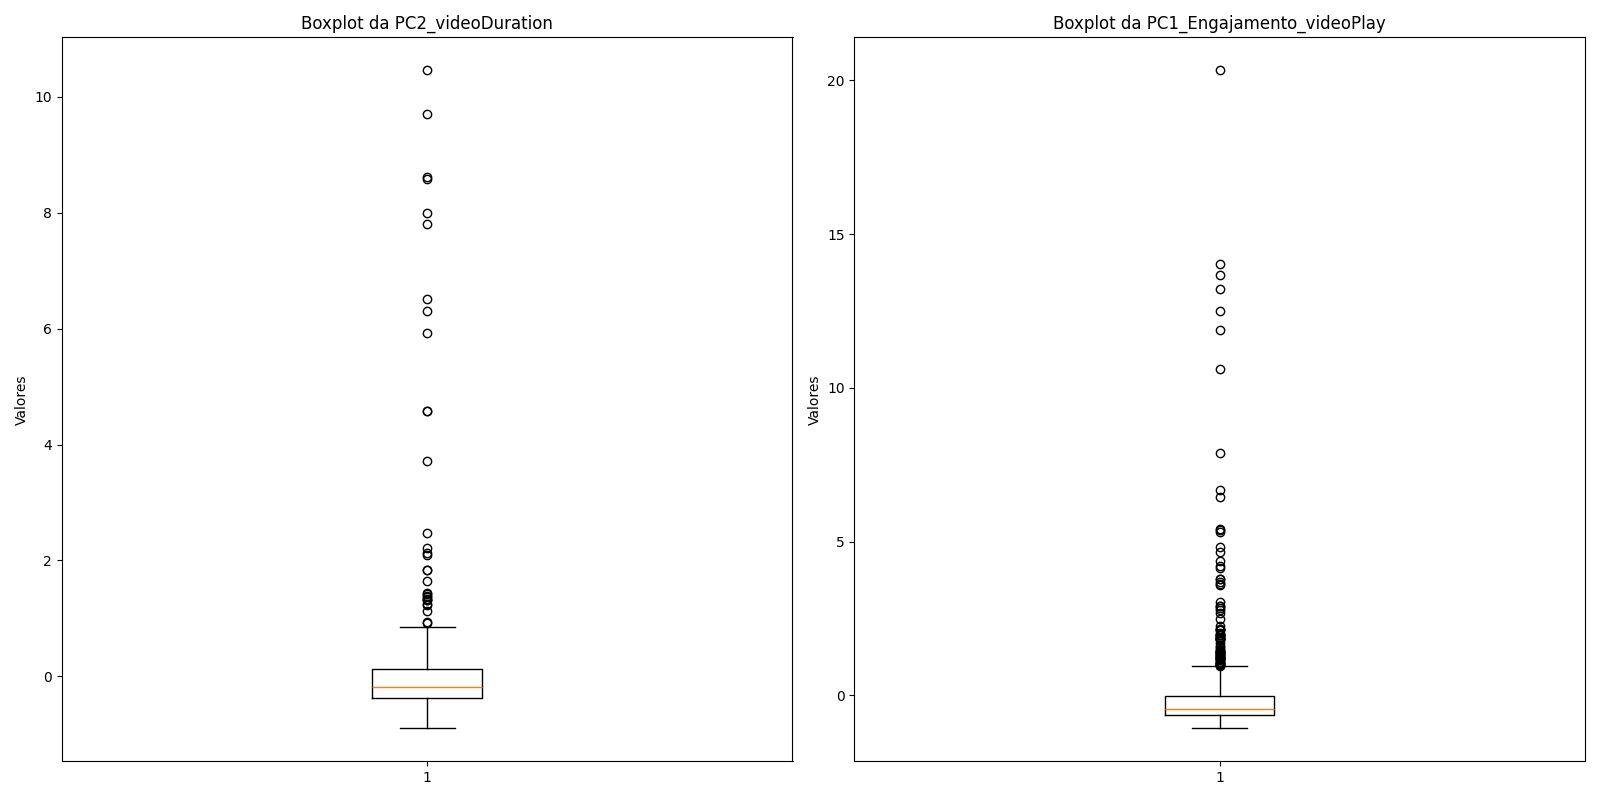
\includegraphics[width=1\textwidth]{Figuras/boxplot_do_dataframe.png}
    \caption{Boxplot dos Componentes Principais PC1 (Engajamento) e PC2 (Duração).}
    \label{fig:boxplot_pca}
\end{figure}

 O gráfico à direita, representando o PC1 (Engajamento\_videoPlay), revela que a grande maioria dos Reels possui um nível de engajamento concentrado em torno da mediana, que está próxima de zero. No entanto, a presença de uma longa cauda de outliers positivos, com valores que ultrapassam 20, é notável e característica de dados de engajamento, indicando que um número restrito de vídeos alcançou uma viralidade significativamente superior à média. De forma análoga, o gráfico à esquerda para o PC2 (videoDuration) mostra que a maioria dos vídeos tem uma duração padronizada e curta, também com uma cauda de outliers positivos que representam vídeos excepcionalmente mais longos. A existência proeminente de outliers em ambos os componentes sugere que tanto o engajamento viral quanto os vídeos de longa duração são eventos atípicos no conjunto de dados, o que justifica a utilização de algoritmos de clusterização robustos a outliers, como o DBSCAN, na etapa subsequente da análise.

\section{Clusterização}

Com base nos dois componentes principais, foi utilizada a ferramenta \texttt{AutoClusterHPO} para determinar o algoritmo de clusterização mais adequado. A ferramenta identificou o \textbf{DBSCAN} como o melhor algoritmo, com os parâmetros \texttt{eps=1.40} e \texttt{min\_samples=5}. O DBSCAN é um algoritmo baseado em densidade que é eficaz na identificação de clusters de formas arbitrárias e na detecção de outliers. A clusterização resultou em três grupos principais, como visualizado na Figura \ref{fig:clusters_pca}. A maioria dos Reels (792) foi agrupada no Cluster 0, enquanto 12 foram classificados como outliers (Cluster -1) e um pequeno grupo de 6 Reels formou o Cluster 1.

\begin{figure}[h!]
    \centering
    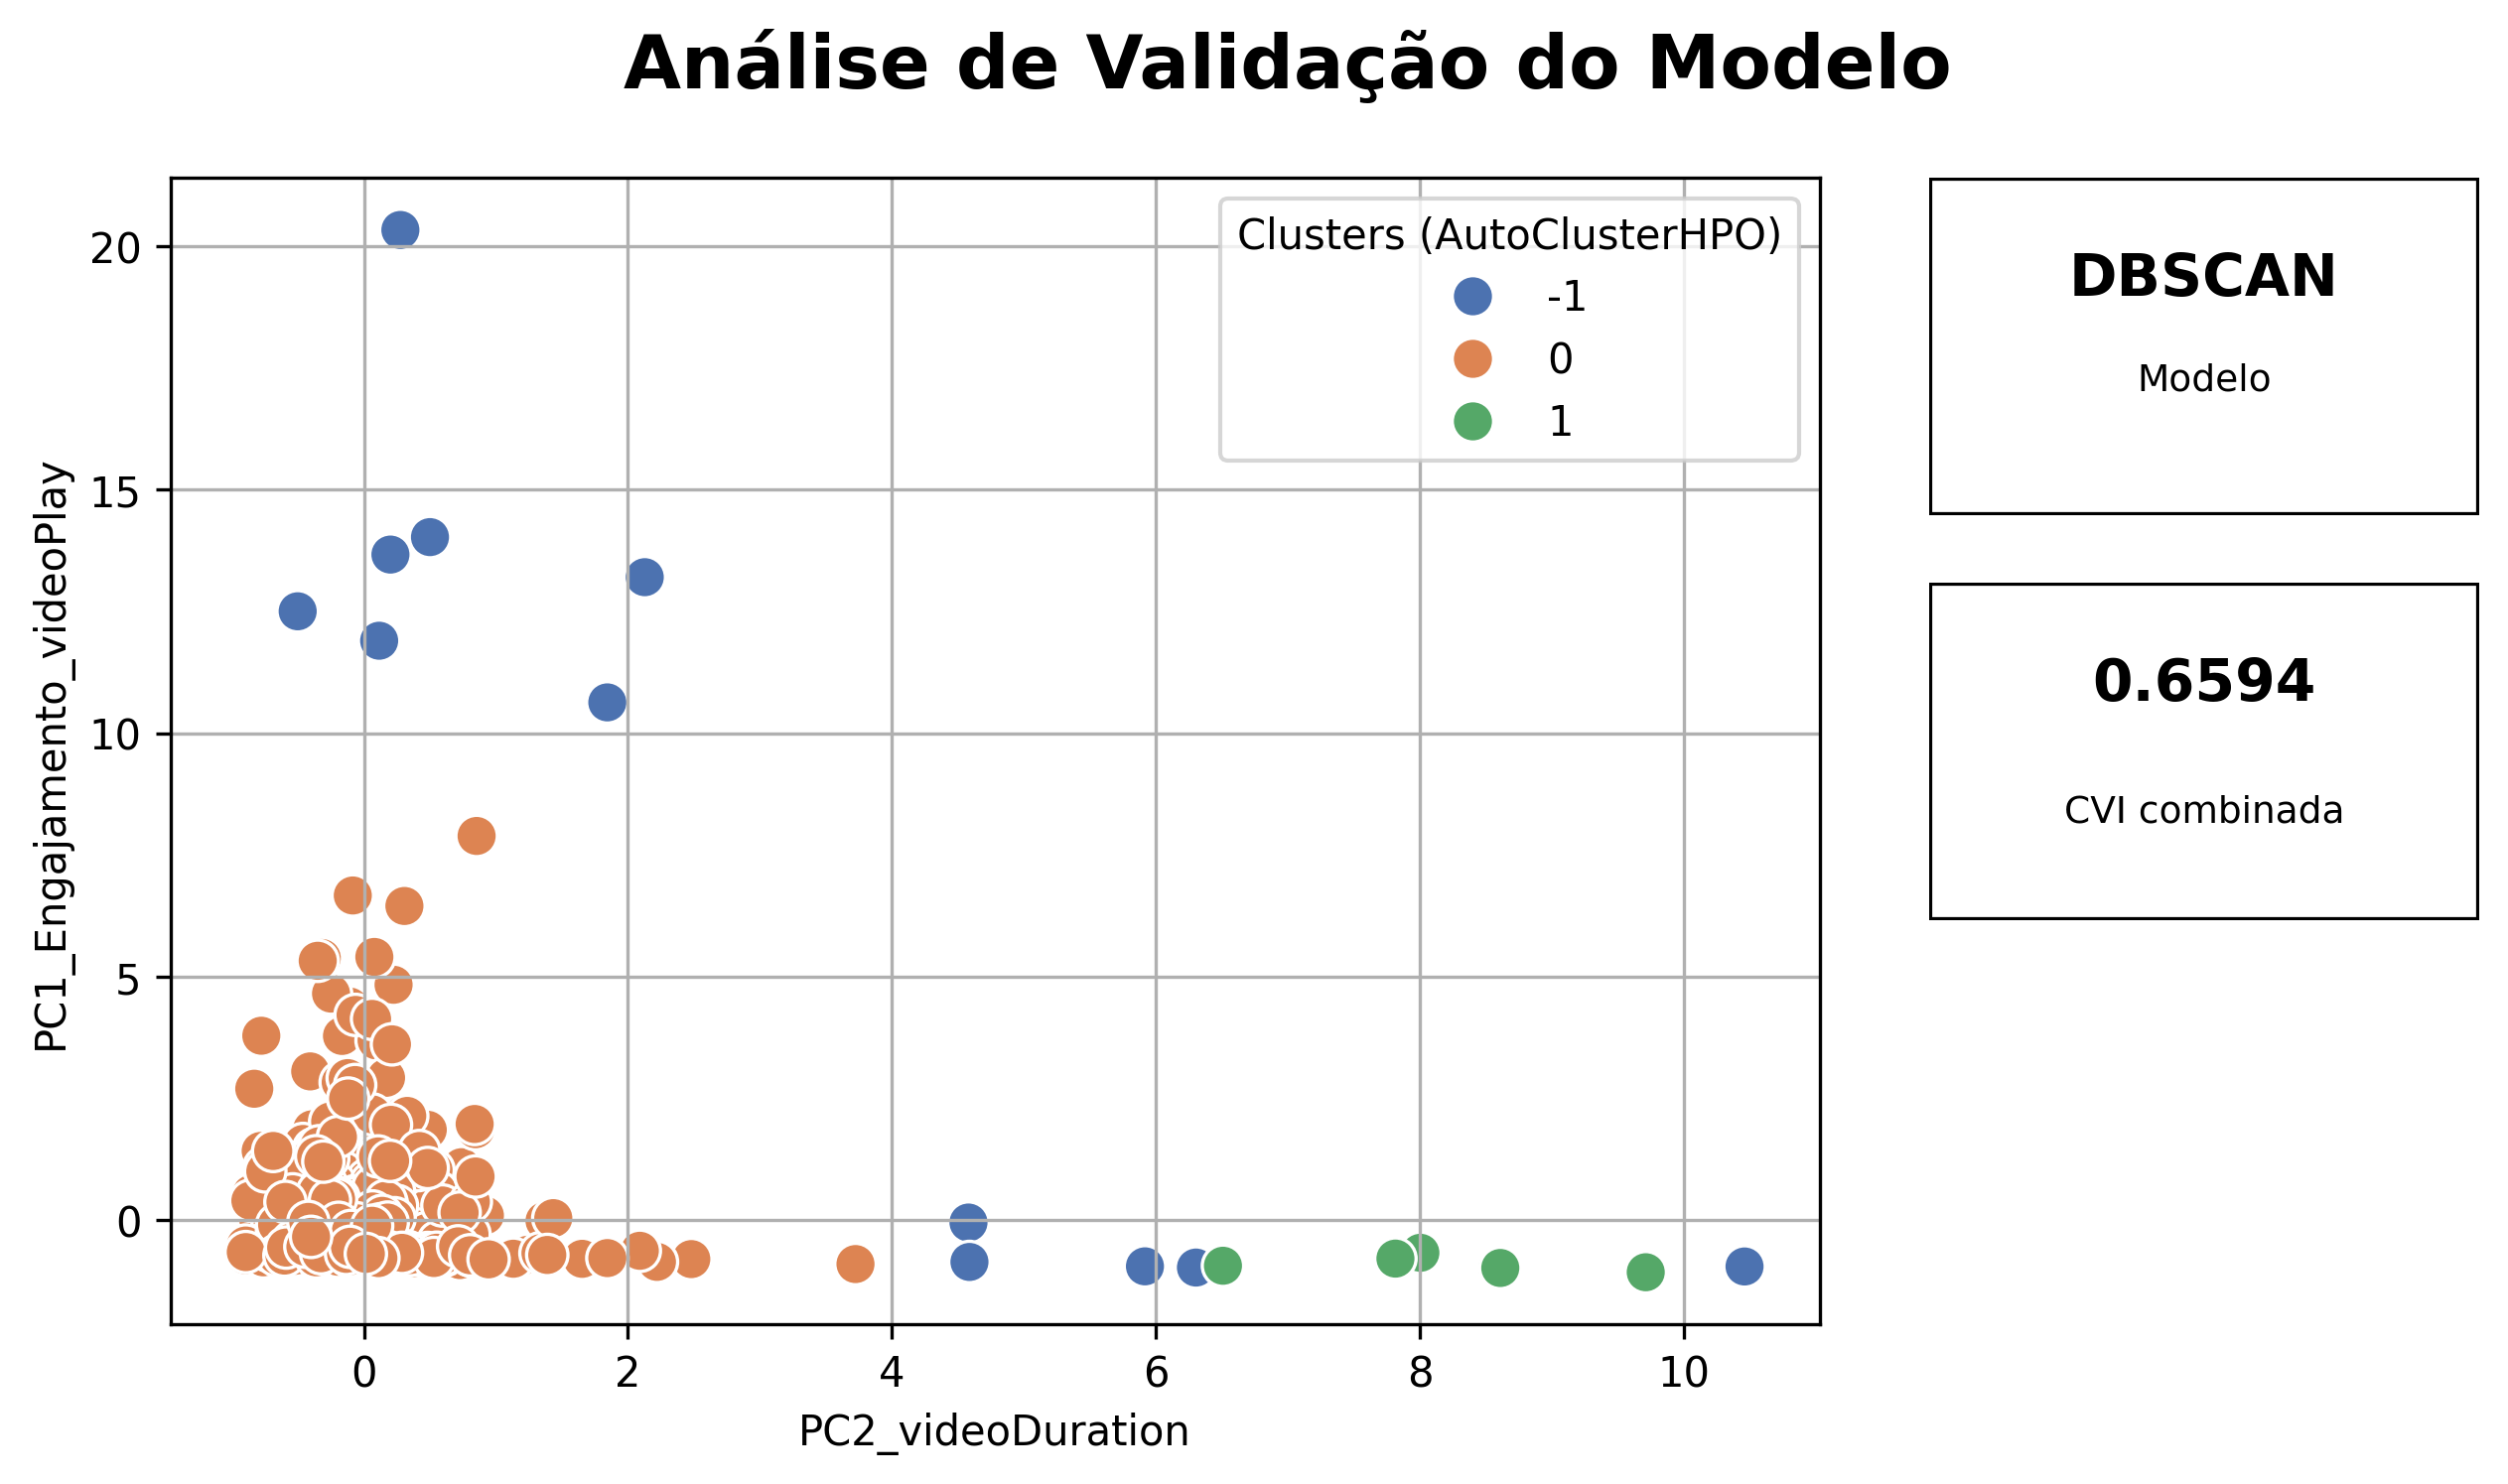
\includegraphics[width=1\textwidth]{Figuras/avaliacaoAutoCluster.png}
    \caption{Visualização dos Clusters com base nos Componentes Principais.}
    \label{fig:clusters_pca}
\end{figure}

A aplica\c{c}\~ao do framework \textit{AutoClusterHPO} para a an\'alise de dados dos Reels do Instagram, conforme visualizado na Figura 2, culminou na sele\c{c}\~ao autom\'atica do algoritmo DBSCAN como o modelo \'otimo, alcan\c{c}ando uma pontua\c{c}\~ao CVI combinada de 0.6594. A distribui\c{c}\~ao dos dados com base nos componentes principais revela uma segmenta\c{c}\~ao coesa, onde o modelo identificou dois clusters principais e um conjunto de outliers (r\'otulo -1). O cluster majorit\'ario (r\'otulo 0) agrupa os v\'ideos com menor dura\c{c}\~ao e engajamento, representando o comportamento padr\~ao na plataforma. De forma not\'avel, os pontos classificados como ru\'ido (-1) podem ser dividios em dois grupos, aqueles com valores elevados no componente principal associado ao engajamento (PC1) com baixa duração e aqueles com baixo engajamento e alta duração, indicando que o m\'etodo foi eficaz em isolar automaticamente os Reels de performance an\^omala.

O Cluster -1, embora contenha apenas 12 observações, contém os Reels de maior impacto. Uma de suas característica mais proeminente são a presença de vídeos com as métricas de engajamento elevadas, com uma média de 4.843 comentários e quase 90.000 curtidas, apesar de 25\% das publicações com menor engajamento apresentarem menos do que 103 comentários. O número de visualizações acompanha essa tendência, com uma média de 1,12 milhão. A duração dos vídeos neste cluster é bastante variada, com os vídeos variando desde 26 até 900 segundos. Mesmo com essa variação, foi possível analisar que os vídeos que contém mais do que 10 de PC1 apresentarem 83.44 segundos de média, variando de 26.32 até 180.03.

Representando a esmagadora maioria dos dados com 792 Reels, o Cluster 0 pode ser definido como o comportamento padrão da plataforma. Sua principal característica é a curta duração dos vídeos, com uma média de apenas 64,5 segundos. O engajamento é moderado e consistente com o que se esperaria de um conteúdo comum: uma média de 408 comentários, 5.543 curtidas e 117.883 visualizações. A baixa variabilidade na duração indica que este grupo é composto majoritariamente por vídeos curtos e rápidos.

O Cluster 1 é o menor grupo, com apenas 6 vídeos, e possui um perfil muito distinto. Sua característica definidora é a duração extremamente longa, com uma média de 721 segundos (aproximadamente 12 minutos). Em contrapartida, este cluster apresenta as piores métricas de desempenho. O engajamento é mínimo, com médias de 184 comentários e 1.554 curtidas, e o número de visualizações é o mais baixo de todos, com uma média de 29.323, sugerindo que vídeos muito longos no formato Reels não conseguem reter a atenção do público.

A principal diferença entre os clusters reside na aparente relação entre a duração do vídeo e o engajamento. O Cluster 0, de vídeos curtos, estabelece uma base de desempenho moderado, enquanto o Cluster 1 demonstra que estender excessivamente a duração leva a uma queda drástica no desempenho. Em contraste, o Cluster -1 mostra que o conteúdo de alto impacto pode performar excepcionalmente bem, com métricas de engajamento que são de 10 a 20 vezes maiores que as do Cluster 0.

Apesar das diferenças marcantes, uma semelhança notável pode ser encontrada na distribuição dos dados de engajamento dentro de cada cluster. Em todos os três grupos, a média de comentários e curtidas é consistentemente superior à mediana. Isso indica uma assimetria positiva em todos os segmentos, sugerindo que, mesmo dentro de um mesmo perfil de cluster, uma pequena parcela de vídeos tende a performar significativamente melhor que a maioria, criando uma "cauda longa" de popularidade.

\section{Análise de Sentimentos}

Para a classificação de sentimentos, foi utilizado um modelo pré-treinado robusto, o \texttt{cardiffnlp/twitter-xlm-roberta-base-sentiment}, através da biblioteca Transformers. Este modelo é especializado em textos de redes sociais e classifica cada comentário em uma de três categorias: \texttt{positive}, \texttt{neutral} ou \texttt{negative}. Além do rótulo, o modelo fornece um \textbf{score de confiança} (de 0 a 1), que indica o grau de certeza da classificação. 

A análise de sentimentos realizada neste projeto revelou uma predominância massiva de comentários positivos. As distribuições foram as seguintes:

\begin{figure}[h!]
    \centering
    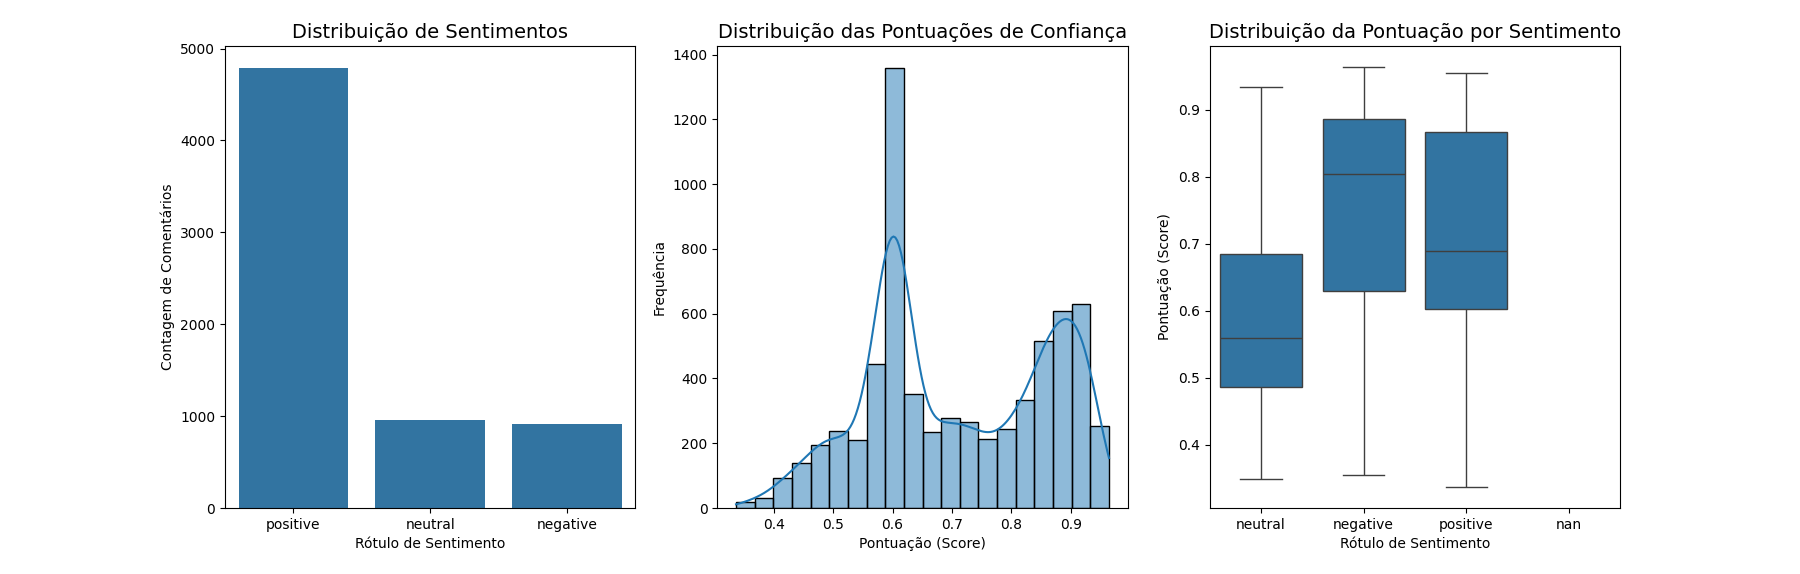
\includegraphics[width=\textwidth]{Figuras/sentiment_plots.png} 
    \caption{Visualizações da Análise de Sentimento: (a) Distribuição de Rótulos, (b) Distribuição dos Scores de Confiança, (c) Boxplot de Scores por Sentimento.}
    \label{fig:sentiment}
\end{figure}

Acima, é possível analisar que o Histograma de Scores de Confiança mostra que o modelo realizou a maioria de suas classificações com alta confiança (scores próximos de 1.0), indicando robustez. O Boxplot detalha essa confiança por categoria, mostrando que as classificações \texttt{positive} e \texttt{negative} possuem scores consistentemente mais altos do que a categoria \texttt{neutral}, o que é esperado, já que a neutralidade é semanticamente mais ambígua.

\subsection{Análise de Sentimentos por Perfis}

Após estabelecer o perfil de sentimento agregado do dataset e analisar a recepção qualitativa dentro dos clusters de performance, esta subseção avança a análise para o nível individual de cada perfil. O objetivo é dissecar a distribuição dos dados e identificar os outliers de performance qualitativa, movendo-se da análise de clusters para a de casos específicos. Ao isolar e examinar os cinco governadores com os maiores percentuais de comentários positivos e, em contrapartida, os cinco com os maiores percentuais de comentários negativos, esta análise busca validar empiricamente a tese central da Análise Exploratória de Dados (AED): a de que o desempenho digital é marcado por uma heterogeneidade extrema. Esta abordagem permite identificar quais figuras públicas específicas estão nas pontas da distribuição, ilustrando os perfis de comunicação que geram maior aprovação ou maior atrito público.

\begin{figure}[h!]
    \centering
    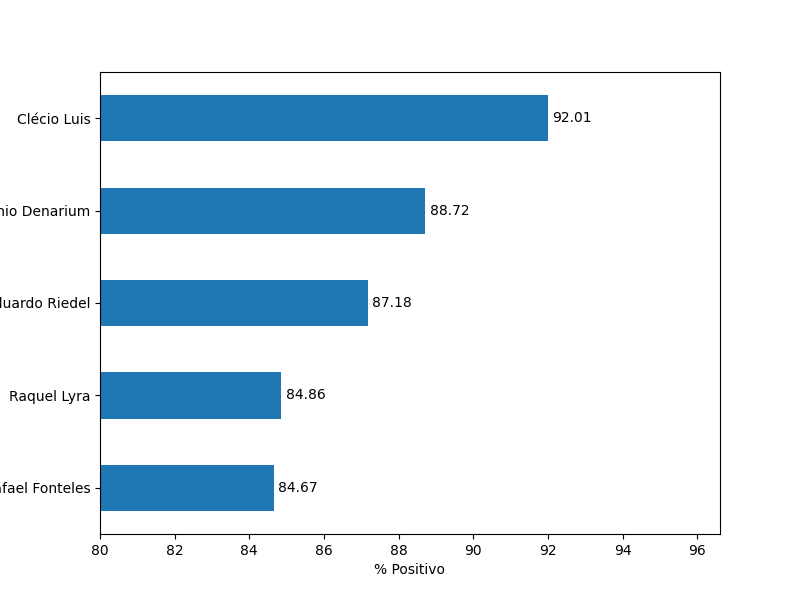
\includegraphics[width=0.5\textwidth]{Figuras/top_5_governadores_positivo.png} 
    \caption{Visualizações da Análise de Sentimento: 5 governadores com Maior percentual de comentários Positivos}
    \label{fig:sentiment}
\end{figure}

A análise do gráfico de barras horizontais, que ilustra os cinco governadores com maior percentual de comentários positivos, revela um desempenho de recepção qualitativa notavelmente elevado para este grupo de elite. Clécio Luís lidera o ranking de forma destacada, com 92,01\% dos comentários em suas publicações classificados como positivos, estabelecendo uma vantagem de mais de 3,2 pontos percentuais sobre o segundo colocado, Antonio Denarium (88,72\%). O grupo dos cinco primeiros é completado por Eduardo Riedel (87,18\%), Raquel Lyra (84,86\%) e Rafael Fonteles (84,67\%). É notável que todos os governadores neste top 5 mantêm um índice de positividade acima de 84\%, um patamar extremamente alto. Este resultado dialoga diretamente com a Análise Exploratória de Dados (AED) apresentada anteriormente na TCC (seção 5.1.1). A AED já havia estabelecido a presença de heterogeneidade extrema e assimetria positiva em todas as métricas quantitativas, como número de seguidores , soma de comentários e taxa de engajamento. Este novo gráfico de sentimento comprova que a mesma variabilidade se aplica à recepção qualitativa: assim como a AED identificou outliers quantitativos que distorcem a média (perfis com desempenho muito acima do padrão), o desempenho de Clécio Luís (92,01\%) representa um outlier qualitativo, validando a conclusão do TCC de que o desempenho dos governadores no Instagram não é uniforme, mas sim caracterizado por picos de performance excepcionais que se distanciam significativamente da mediana.

\begin{figure}[h!]
    \centering
    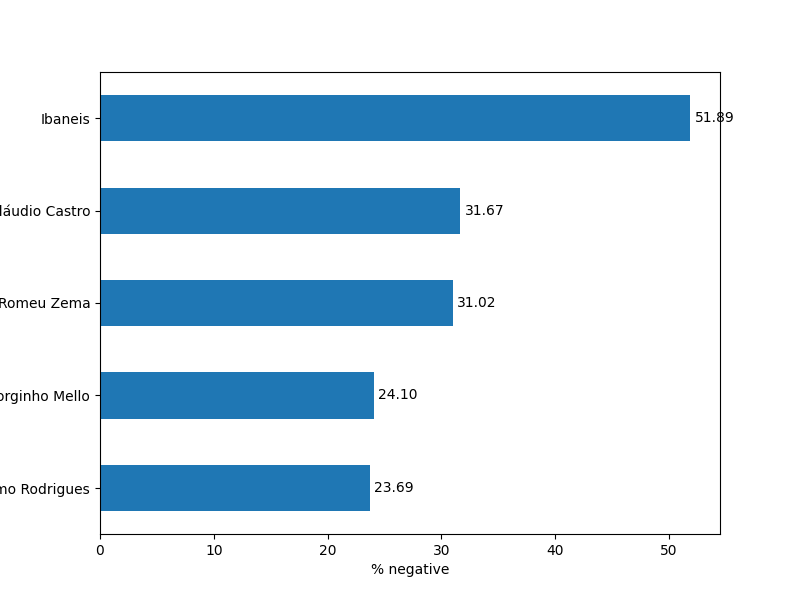
\includegraphics[width=0.5\textwidth]{Figuras/top_5_governadores_negativo.png} 
    \caption{Visualizações da Análise de Sentimento: Visualizações da Análise de Sentimento: 5 governadores com Maior percentual de comentários Negativos}
    \label{fig:sentiment}
\end{figure}

Em contrapartida, a análise dos cinco governadores com maior percentual de comentários negativos expõe o outro extremo da recepção pública. O governador Ibaneis apresenta-se como um outlier negativo proeminente, com 51,89\% de seus comentários classificados como negativos, indicando que mais da metade das interações em seu perfil são críticas. Este resultado é drasticamente superior aos demais, com Cláudio Castro (31,67\%) e Romeu Zema (31,02\%) formando um segundo patamar, seguidos por Jorginho Mello (24,10\%) e Tino Rodrigues (23,69\%). A existência de um perfil cuja recepção negativa supera os 50\% é uma ilustração clara da heterogeneidade extrema e da distribuição assimétrica que a Análise Exploratória de Dados (AED) do TCC (seção 5.1.1) já havia identificado. Assim como a AED revelou outliers de performance quantitativa (perfis com engajamento muito acima da média), este gráfico valida que também existem outliers qualitativos, onde a recepção do público é significativamente mais hostil do que a do restante do grupo, reforçando a conclusão de que o desempenho digital dos governadores é marcado por extremos em ambas as pontas.

A análise dos extremos da recepção qualitativa oferece uma conclusão contundente: a performance de sentimento dos governadores é tão ou mais assimétrica do que suas métricas de engajamento. A existência de um perfil como o de Clécio Luís, que alcança uma aprovação quase universal (92,01\% positiva), em conjunto com um perfil como o de Ibaneis, onde a hostilidade é majoritária (51,89\% negativa), invalida a noção de um "desempenho médio". Estes resultados reforçam de maneira inequívoca os achados da AED, demonstrando que o cenário digital não é um ambiente homogêneo, mas sim um conjunto de "microclimas" de recepção altamente polarizados. Fica evidente que o sucesso ou o fracasso na comunicação digital não se mede apenas pela quantidade de interações, mas pela qualidade drasticamente distinta dessa recepção, que varia de aprovação esmagadora a uma rejeição majoritária.

\subsection{Análise de Sentimentos por Clusters}

Para aprofundar a compreensão dos padrões de desempenho identificados, esta seção avança da segmentação métrica para a qualificação emocional, integrando os resultados da clusterização (seção 5.3) com os da análise de sentimentos (seção 5.4). Não basta identificar os clusters "Padrão" (Cluster 0), "Viral" (Cluster -1) e "Longo/Baixa Performance" (Cluster 1); é crucial dissecar a natureza da recepção do público dentro de cada um desses grupos. O objetivo desta análise cruzada é, portanto, mapear a distribuição percentual de comentários positivos, neutros e negativos para cada cluster. Esta abordagem sinérgica permite validar as características de cada grupo, revelando se a performance viral está associada à aclamação ou à controvérsia, e se a baixa performance está ligada à indiferença ou à rejeição

\begin{figure}[h!]
    \centering
    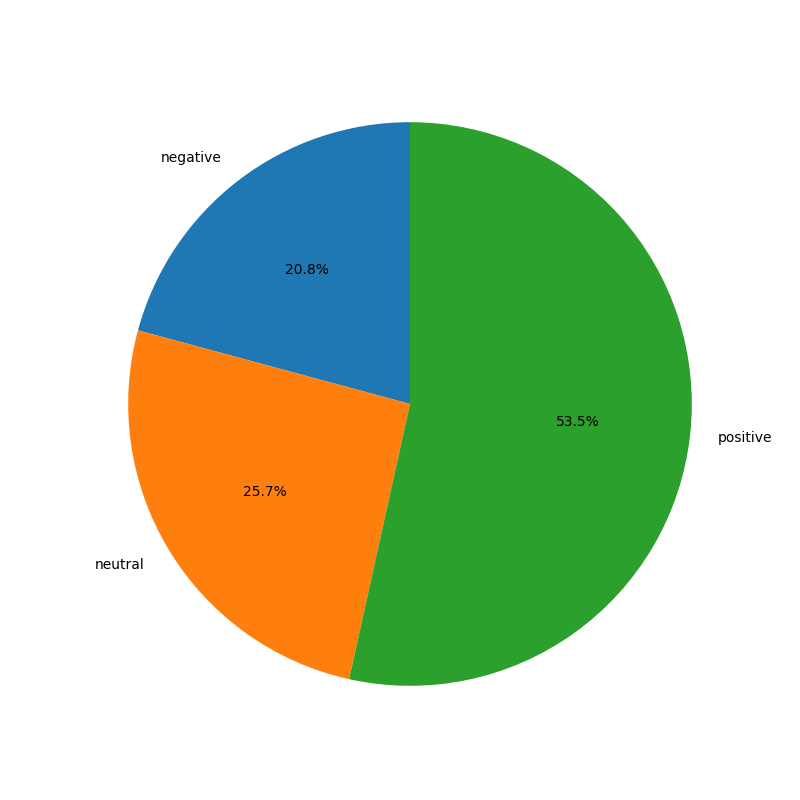
\includegraphics[width=0.4\textwidth]{Figuras/grafico_sentimentos_cluster-1.png} 
    \caption{Visualizações da Análise de Sentimento: Distribuição de Rótulos (Cluster -1)}
    \label{fig:sentiment}
\end{figure}

A análise de sentimentos para o Cluster -1, que o TCC identificou como o grupo de 12 Reels "outliers" de alto impacto e viralidade, revela uma dinâmica de recepção muito mais polarizada em comparação ao Cluster 0. Embora os comentários positivos ainda sejam majoritários (53,5\%), essa proporção é substancialmente menor (em comparação aos 72,3\% do Cluster 0). O insight mais relevante é o crescimento expressivo das reações não-positivas: os comentários negativos (20,8\%) e neutros (25,7\%) somam 46,5\% do total. Isso sugere que o conteúdo viral, caracterizado por um "Índice de Engajamento" (PC1) anômalo, não gera apenas aprovação, mas também atrai um volume significativamente maior de debate, críticas e reações ambíguas, refletindo a natureza muitas vezes controversa ou divisiva que impulsiona a própria viralidade.


\begin{figure}[h!]
    \centering
    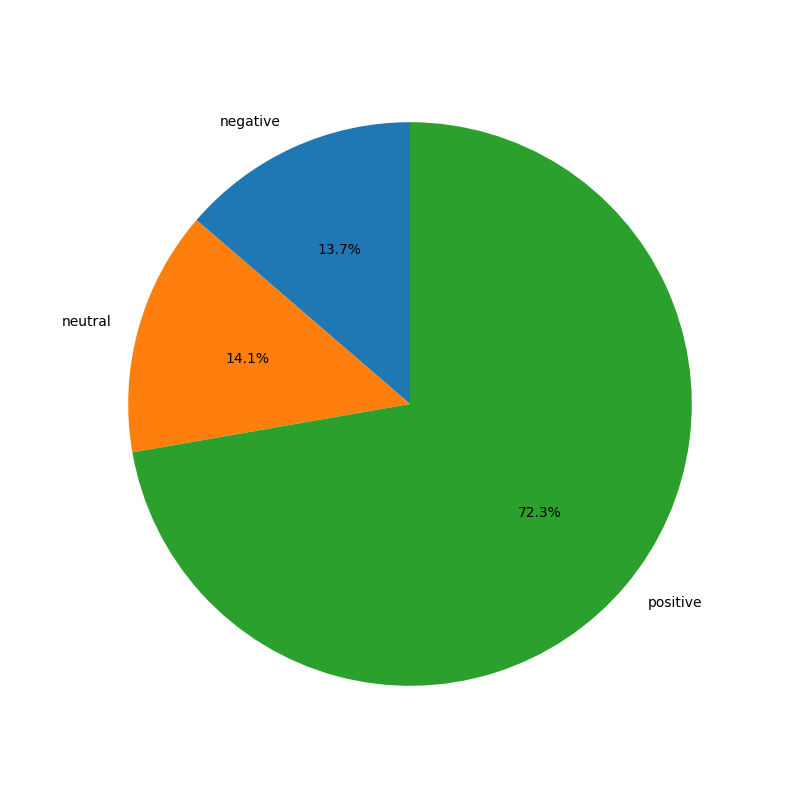
\includegraphics[width=0.4\textwidth]{Figuras/grafico_sentimentos_cluster0.png} 
    \caption{Visualizações da Análise de Sentimento: Distribuição de Rótulos (Cluster 0)}
    \label{fig:sentiment}
\end{figure}

A análise de sentimentos detalhada para o Cluster 0, o grupo mais representativo com 792 Reels, revela que o conteúdo "padrão" da plataforma é recebido de forma esmagadoramente positiva. Conforme o gráfico de pizza, 72,3\% dos comentários associados a este cluster foram classificados como positivos, indicando uma forte aprovação. Os sentimentos neutros (14,1\%) e negativos (13,7\%) são minoritários e apresentam proporções quase idênticas. Este resultado complementa e enriquece a definição anterior do Cluster 0: que os vídeos definidos pelo seu desempenho métrico "padrão" (curta duração, com média de 64,5 segundos, e engajamento moderado)  geram, de forma consistente, uma resposta emocional majoritariamente favorável do público.

\begin{figure}[h!]
    \centering
    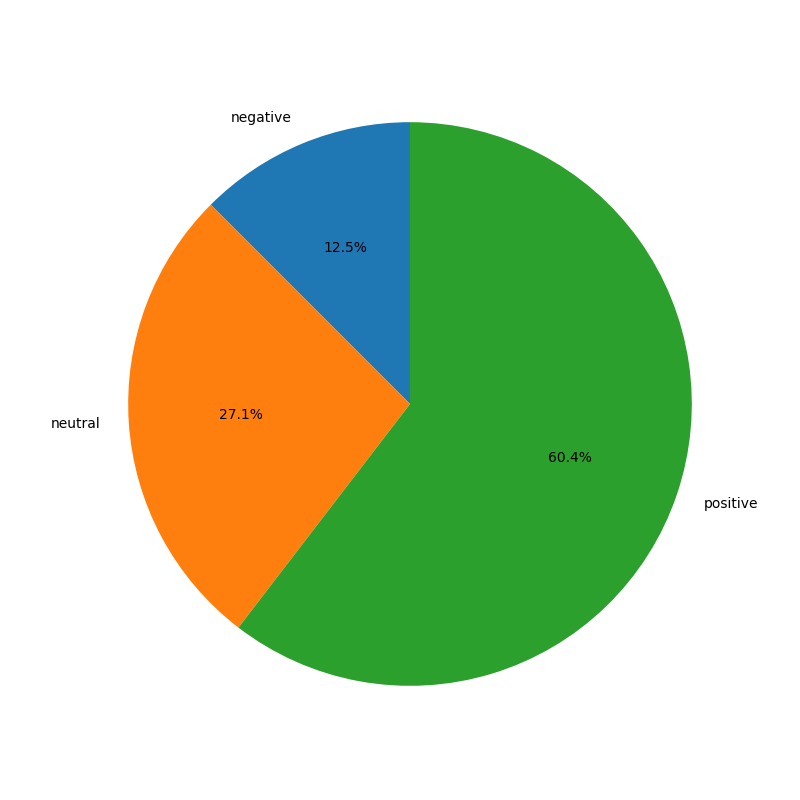
\includegraphics[width=0.4\textwidth]{Figuras/grafico_sentimentos_cluster1.png} 
    \caption{Visualizações da Análise de Sentimento: Distribuição de Rótulos (Cluster 1)}
    \label{fig:sentiment}
\end{figure}

A análise de sentimentos para o Cluster 1, o grupo de 6 Reels definido por sua duração extrema (média de 721 segundos) e desempenho de engajamento muito baixo, apresenta um perfil de recepção peculiar. Embora os comentários positivos ainda sejam a maioria (60,4\%), o dado mais distintivo é a alta proporção de comentários neutros (27,1\%), a maior entre todos os clusters. Combinado com o menor índice de comentários negativos (12,5\%), isso sugere um padrão claro: esses vídeos longos, que o TCC já havia identificado como de baixa performance, parecem falhar em gerar reações fortes. Eles não geram o alto engajamento do Cluster -1, mas também não atraem a negatividade; em vez disso, a audiência que interage é ou levemente positiva ou, mais significativamente, neutra, o que reforça a conclusão de que o conteúdo não consegue reter a atenção ou provocar um debate engajado, alinhando-se perfeitamente com suas métricas de desempenho fracas.

Com isso, conclui-se que a integração da análise de sentimentos com a clusterização é fundamental para desmistificar o real significado da performance métrica. Os resultados demonstram que "alto engajamento" não é sinônimo de "alta aprovação". O Cluster 0 (Padrão) estabelece a linha de base com uma recepção esmagadoramente positiva (72,3\%). Em nítido contraste, o Cluster -1 (Viral), dono das métricas mais fortes, revela-se o mais polarizado, com uma maioria positiva reduzida (53,5\%) e as maiores taxas de comentários negativos (20,8\%) e neutros (25,7\%), indicando que a viralidade foi impulsionada tanto pela aclamação quanto pela controvérsia. Por fim, o Cluster 1 (Longo/Baixa Performance) confirma sua ineficácia  ao apresentar a maior taxa de indiferença (27,1\% de comentários neutros), falhando em gerar reações emocionais fortes. A análise híbrida, portanto, qualifica os clusters, provando que o conteúdo padrão é aprovado, o viral é debatido, e o longo é ignorado.

\section{Modelagem de Tópicos com BERTopic}

A modelagem de tópicos identificou 50 temas distintos no corpus. As visualizações interativas fornecem insights profundos sobre a estrutura desses temas. O mapa da Figura 4 (Intertopic Distance Map) abaixo posiciona os tópicos em um espaço 2D com base em sua similaridade semântica. Cada círculo representa um tópico, e seu tamanho é proporcional à sua frequência.

\begin{figure}[h!]
    \centering
    % Substitua 'intertopic_map.png' pelo nome do arquivo de imagem salvo do seu notebook.
    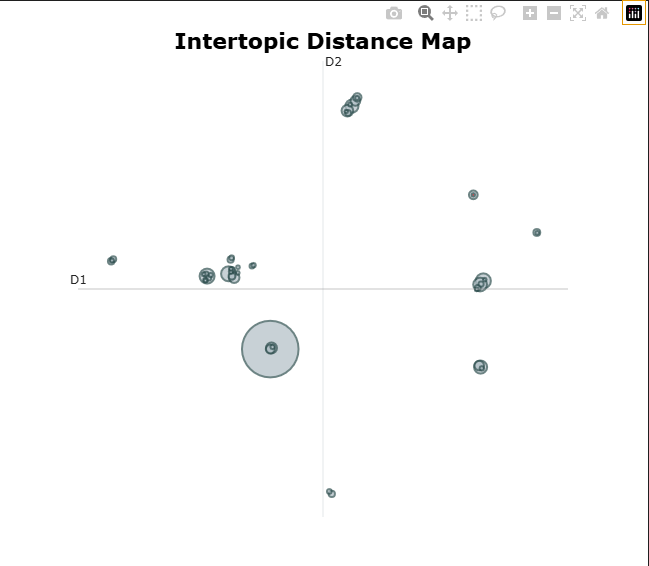
\includegraphics[width=0.9\textwidth]{Figuras/intertopic_map.png}
    \caption{Mapa de Distância Intertópica. Círculos próximos são semanticamente similares.}
    \label{fig:intertopic}
\end{figure}

A análise do mapa revela um \textbf{tópico dominante} (círculo grande), que representa a maioria dos comentários e é composto principalmente por expressões de apoio e emojis positivos (ex: aplausos, corações). Os demais tópicos, menores e mais dispersos, formam clusters que abordam assuntos mais específicos, como política, críticas a serviços públicos e pedidos de justiça.

Já o dendrograma de clusterização hierárquica (Figura 5) e o mapa de calor de similaridade (Figura 6) complementam a análise, mostrando como os tópicos se relacionam e podem ser agregados em meta-tópicos. Por exemplo, tópicos relacionados a críticas sobre concursos públicos e serviços de saúde, embora distintos, mostram-se semanticamente próximos e poderiam ser agrupados sob um tema maior de "Reivindicações de Serviços Públicos".

\begin{figure}[h!]
    \centering
    % Substitua 'hierarchy.png' pelo nome do arquivo de imagem salvo do seu notebook.
    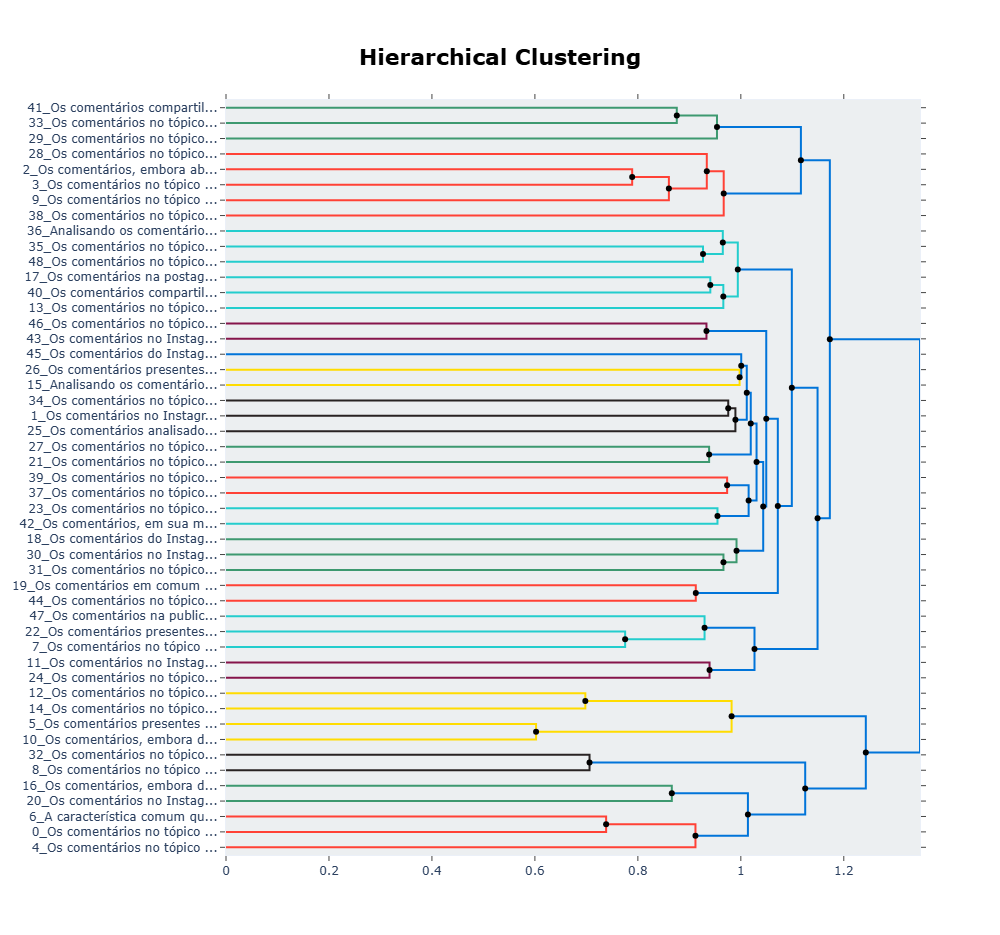
\includegraphics[width=\textwidth]{Figuras/hierarchy.png}
    \caption{Dendrograma da Clusterização Hierárquica dos Tópicos.}
    \label{fig:hierarchy}
\end{figure}

Com base na análise do dendrograma de clusterização hierárquica, a modelagem de tópicos mais coesa e distinta agruparia os comentários em quatro clusters principais. A justificativa para essa escolha reside em observar as distâncias horizontais em que os agrupamentos são formados. Ao traçar uma linha de corte vertical imaginária no eixo de distância em aproximadamente 1.1, identificamos quatro agrupamentos distintos que são fundidos em etapas posteriores com uma distância (dissimilaridade) significativamente maior, indicado pelas longas linhas horizontais que os conectam. O primeiro tópico hierárquico (topo, em tons de verde e vermelho) representa um tópico coeso. O segundo (meio-superior, em ciano, amarelo e preto) é o maior e mais diverso grupo, mas ainda assim claramente distinto dos demais. O terceiro (meio-inferior, em marrom e roxo) e o quarto (base do gráfico, em amarelo, cinza e vermelho) formam os dois últimos tópicos. Esta divisão em quatro grupos otimiza a modelagem, pois maximiza a similaridade dos comentários dentro de cada grupo, ao mesmo tempo que garante que os tópicos sejam significativamente diferentes entre si.

Os itens do primeiro tópico hierárquico (tópicos: 2, 3, 9, 29, 33, 36, 38, 41), têm em comum a descrição de comentários que expressam um forte sentimento de apoio, concordância e aprovação. A análise foca em reações positivas, como elogios a iniciativas e concordância com o conteúdo postado. Além disso, muitos itens descrevem ações que os usuários desejam realizar ou estão com dificuldade para fazer, como encontrar um link para inscrição ou cadastro, o que os une pelo tema de "ação do usuário". Quanto aos itens do segundo tópico hierárquico (tópicos: 1, 17, 21, 23, 25, 26, 28, 34, 35, 37, 39, 40, 42, 43, 45, 46), a principal característica deste grupo é a contextualização. As análises aqui presentes se concentram em identificar a origem dos comentários (plataforma, tipo de postagem) e frequentemente mencionam figuras de autoridade, como governadores, políticos ou outras personalidades públicas. O tema central é descrever a quem os comentários se dirigem e de onde vêm. Já os itens do terceiro tópico hierárquico (tópicos: 7, 11, 12, 14, 18, 19, 22, 24, 30, 31, 44, 47) agrupa as análises que se aprofundam nas qualidades e sentimentos dos comentários. Os textos descrevem o tom (irônico, crítico, de apoio), o estilo da linguagem, e as emoções predominantes, como admiração, insatisfação ou preocupação. O elo comum é a qualificação do discurso, indo além do tema para capturar a nuance e a subjetividade das mensagens. Por fim, os itens do quarto tópico hierárquico (tópicos: 4, 5, 6, 8, 10, 16, 20, 27, 32) são unidos por um forte viés de crítica, insatisfação e debate. As análises descrevem comentários que abordam problemas sociais, fazem reclamações, apontam divergências e expressam descontentamento com temas como gestão pública, segurança, educação e corrupção. É o cluster que representa a análise do discurso de oposição e conflito.

Abaixo pode-se analisar a matriz de similaridade entre os tópicos, que de forma semelhante ao dendograma, permitirá ao projeto agrupar tópicos semelhantes entre si. 

\begin{figure}[h!]
    \centering
    % Substitua 'heatmap.png' pelo nome do arquivo de imagem salvo do seu notebook.
    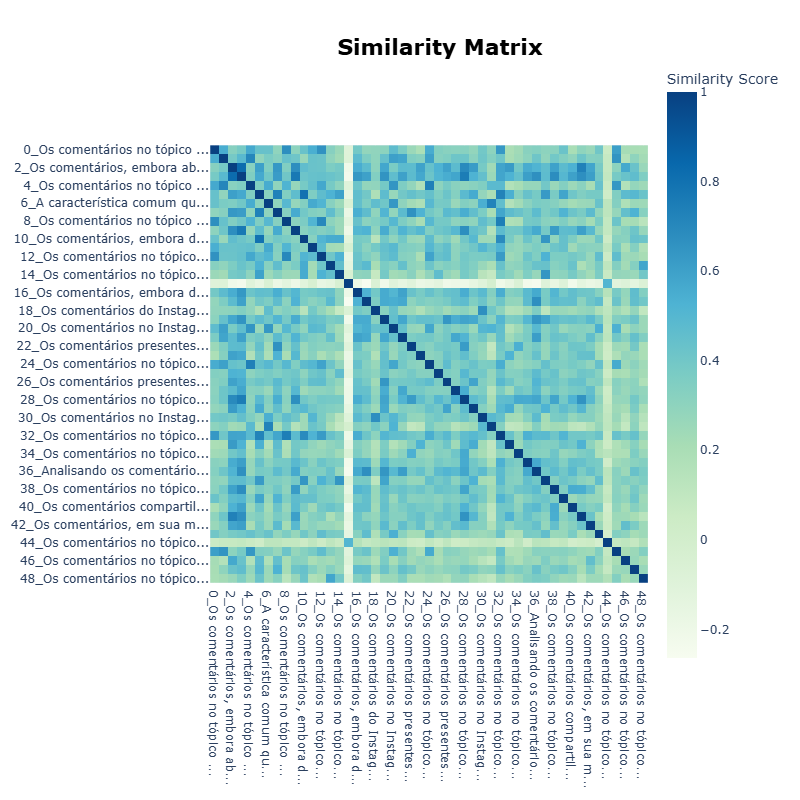
\includegraphics[width=\textwidth]{Figuras/heatmap.png}
    \caption{Matriz de Similaridade (Heatmap) entre os Tópicos.}
    \label{fig:heatmap}
\end{figure}

Analisando a matriz de similaridade, a modelagem de tópicos agruparia os comentários em aproximadamente quatro clusters principais, que são visualmente identificáveis como "quadrados" de cores mais escuras (tons de azul) ao longo da diagonal. A lógica para essa divisão é que os itens dentro de cada um desses quadrados demonstram uma alta pontuação de similaridade mútua, indicando que compartilham o mesmo tema central. O primeiro agrupamento pode ser visto no canto superior esquerdo (itens 0 a 8). Um segundo grupo coeso é observável no meio da matriz (aproximadamente itens 20 a 26). Um terceiro cluster é notado logo abaixo (itens 30 a 36). Finalmente, o agrupamento mais forte e coeso parece ser o do canto inferior direito (itens 40 a 48), que exibe os tons de azul mais escuros e consistentes, sugerindo uma altíssima similaridade interna. As áreas de cores mais claras (verdes/amarelas) entre esses blocos azuis representam a baixa similaridade entre os diferentes tópicos, justificando a sua separação em grupos distintos.

A aplicação do pipeline híbrido de NLP revelou com sucesso as principais características do corpus de comentários do Instagram. A análise de sentimentos indicou uma recepção majoritariamente positiva ao conteúdo dos Reels, com alta confiança do modelo classificador.

A modelagem de tópicos híbrida, combinando BERTopic e Gemini, provou ser excepcionalmente eficaz. Ela não apenas identificou a estrutura temática dos dados—com um tópico principal de reações positivas e diversos subtópicos específicos—mas também forneceu descrições contextuais e de fácil interpretação para cada tema. Esta abordagem representa um avanço significativo em relação aos métodos tradicionais, permitindo uma análise qualitativa mais profunda e a extração de insights acionáveis com maior facilidade. Os resultados demonstram o potencial da integração de modelos de embedding e modelos generativos para análises de texto complexas.

